\documentclass[dvipsnames]{standalone}
\usepackage{tikz}

\usetikzlibrary{positioning}
\usetikzlibrary{calc}

\colorlet{line2line}{SkyBlue!50}

\newcommand{\stheight}{0.7cm}
\newcommand{\stshift}{0.3cm}
\newcommand{\labeloffset}{1.6cm}


\begin{document}

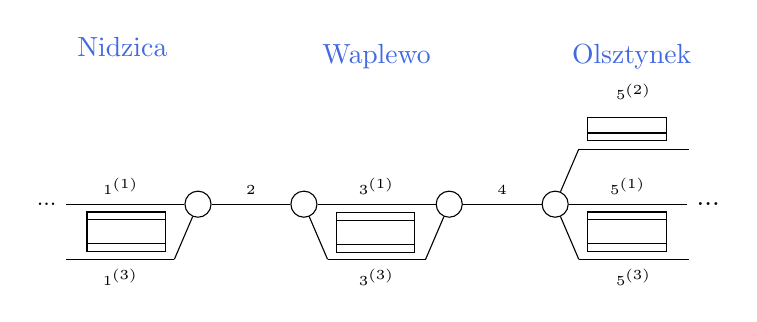
\begin{tikzpicture}[
    junction/.style={draw,circle},
    station/.style={text=RoyalBlue},
    onesideplatform/.pic={
        \node[
            draw,rectangle,minimum height=0.3cm, minimum width=1cm
        ] (platform) {};
        \coordinate [below=0.05cm of platform.west] (x);
        \coordinate [below=0.05cm of platform.east] (y);
        \draw (x) -- (y);
    },
    twosideplatform/.pic={
        \node[
            draw,rectangle,minimum height=0.5cm, minimum width=1cm
        ] (platform) {};
        \coordinate [above=0.15cm of platform.west] (x);
        \coordinate [above=0.15cm of platform.east] (y);
        \coordinate [below=0.15cm of platform.west] (u);
        \coordinate [below=0.15cm of platform.east] (v);
        \draw (x) -- (y);
        \draw (u) -- (v);
    }
]

\node [] (start) {\footnotesize ...};
\node [junction, right=1.5cm of start] (A) {};
\node [junction, right=1cm of A] (B) {};
\node [junction, right=1.5cm of B] (C) {};
\node [junction, right=1cm of C] (D) {};
\node [right=1.5cm of D] (stop) {...};
\node [station,above=\labeloffset of $(start.north)!0.5!(A.north)$] {Nidzica};
\node [station,above=\labeloffset of $(B)!0.5!(C)$] {Waplewo};
\node [station,above=\labeloffset of $(D)!0.5!(stop)$] {Olsztynek};

 \draw (start) -- (A) node[midway,above left=0.0cm and -0.29cm]{\tiny $1^{(1)}$};
\draw (A) -- (B) node[midway,above]{\tiny $2$};
\draw (B) -- (C) node[midway,above]{\tiny $3^{(1)}$};
\draw (C) -- (D) node[midway,above]{\tiny $4$};
\draw (D) -- (stop) node[midway,above]{\tiny $5^{(1)}$};

\coordinate [below right=\stheight and 0.25cm of start.center] (start1);
\coordinate [below left=\stheight and \stshift of A.center] (A1);
\draw (start1) -- (A1) node[midway, below]{\tiny $1^{(3)}$};
\draw (A1) -- (A);


\coordinate [below right=\stheight and \stshift of B.center] (B1);
\coordinate [below left=\stheight and \stshift of C.center] (C1);
\draw (B) -- (B1);
\draw (B1) -- (C1) node[midway,below]{\tiny $3^{(3)}$};
\draw (C1) -- (C);

\coordinate [below left=\stheight and 0.25cm of stop.center] (stop1);
\coordinate [below right=\stheight and \stshift of D.center] (D1);
\draw (D) -- (D1);
\draw (D1) -- (stop1) node[midway,below]{\tiny $5^{(3)}$};


\coordinate [above left=\stheight and 0.25cm of stop.center] (stop2);
\coordinate [above right=\stheight and \stshift of D.center] (D2);
\draw (D) -- (D2);
\draw (D2) -- (stop2) node[midway,above=0.5cm]{\tiny $5^{(2)}$};

\pic [below left=-0.03cm and 0.28cm of A] {twosideplatform};
\pic [below right=-0.02cm and 0.28cm of B] {twosideplatform};
\pic [below right=-0.03cm and 0.28cm of D] {twosideplatform};
\pic [above right=0.675cm and 0.28cm of D] {onesideplatform};


\end{tikzpicture}


\end{document}
